% NOTE: Gave this presentation on the 19.11.2024.

\documentclass[10pt]{amsart}

\usepackage{algorithm}
\usepackage[noend]{algpseudocode}
\usepackage{amsfonts}
\usepackage{amsmath}
\usepackage{amssymb}
\usepackage{amsthm}
\usepackage[backend=biber, citestyle=numeric-comp, bibstyle=ieee]{biblatex}
\usepackage{changepage}
\usepackage{enumitem}
\usepackage{fancyhdr}
\usepackage{fontspec}
\usepackage{fullpage}
\usepackage[hidelinks]{hyperref}
\usepackage{mathtools}
\usepackage{pgfplots}
\usepgfplotslibrary{colormaps}
\usepackage{physics}
\usepackage{thmtools}
\usepackage{tikz}
\usepackage{tikz-3dplot}
\usetikzlibrary{angles, cd, quantikz2, quotes, patterns}
\usepackage{titlesec}
\usepackage{wasysym}

\usepackage{tikz-cd}

\usepackage{bookmark}
\usepackage[nameinlink]{cleveref}
\usepackage{csquotes}

\pgfplotsset{compat=1.18}

\titleformat{\section}[runin]{\normalsize\bfseries}{\thesection}{1em}{}[]
\titleformat{\subsection}[runin]{\normalsize\bfseries}{\thesubsection}{1em}{}[]
\titleformat{\subsubsection}[runin]{\normalsize\bfseries}{\thesubsubsection}{1em}{}[]

\addbibresource{the_nullspace_projection_lemma.bib}

\theoremstyle{definition}
\newtheorem{theorem}{Theorem}
\newtheorem{definition}{Definition}
\theoremstyle{remark}
\newtheorem{problem}[theorem]{Problem}
\newtheorem{lemma}[theorem]{Lemma}
\newtheorem{remark}[theorem]{Remark}
\newtheorem{observation}[theorem]{Observation}
\newtheorem{example}[theorem]{Example}
\newtheorem{corollary}[theorem]{Corollary}

\renewcommand{\qedsymbol}{\(\blacksquare\)}

\setlength{\parindent}{0pt}

\DeclareMathOperator{\controrot}{CR}
\DeclareMathOperator{\expectation}{E}
\DeclareMathOperator{\gf}{GF}
\DeclareMathOperator{\qft}{QFT}
\DeclareMathOperator{\rk}{rk}
\DeclareMathOperator{\defect}{def}
\DeclareMathOperator{\swapgate}{SWAP}
\DeclareMathOperator{\che}{CHE}
\DeclareMathOperator{\poly}{poly}
\DeclareMathOperator{\Span}{Span}
\DeclareMathOperator{\diag}{diag}

\newcommand{\djk}{\delta_{j, k}}
\newcommand{\tlk}{\tilde{\lambda_k}}

\newcommand{\evalat}[2]{\left.{#1}\middle|\right._{#2}}

% SOURCE: https://tex.stackexchange.com/questions/296151/double-head-and-hook-arrow
\newcommand{\hookdoubleheadrightarrow}{%
    \hookrightarrow\mathrel{\mspace{-15mu}}\rightarrow
}

\newcommand{\draftcomment}[2]{\textcolor{#1}{#2}}

\pgfplotsset{colormap/bluered}
\pgfplotsset{colormap/hot2}
\pgfplotsset{colormap/redyellow}

\begin{document}
    \section*{The Nullspace Projection Lemma} \hfill \hfill valentinpi, Last Change: 19.11.2024

    This short note is dedicated to a small result in the analysis of adiabatic quantum algorithms (AQC), the \emph{Nullspace Projection Lemma}. Let \(m, n \in \mathbb{N}_{\geq 1}\) and \(N \coloneqq 2^n\) throughout.
    
    \phantom{}

    \paragraph*{\textbf{Recap on AQC}} Recall the basic notions from AQC. In a very simple generic framework, we may specify AQC using the following parameters:
    \begin{itemize}
        \item \(n\): Number of qubits.
        \item \(H_0 \in H(N)\): Initial Hamiltonian.
        \item \(H_1 \in H(N)\): Final Hamiltonian.
        \item \(\ket{\psi_0} \in S(\mathbb{C}^N)\): Initial state, a ground state of \(H_0\).
        \item \(H\colon [0, 1] \to H(N)\): Hamiltonian path with \(H(0) = H_0\) and \(H(1) = H_1\).
    \end{itemize}
    There are further parameters such as an employed schedule or incorporated catalyst Hamiltonians. We treat the quantum system as a pair in \(S(\mathbb{C}^N) \times H(N)\). The standard literature has not yet explicitely discussed the requirements on which \(\ket{\psi_0}\) and \(H_0\) can be chosen initially for the ground state of/and the initial Hamiltonian. Based on the current state of the art, we propose the following reasonable convention.

    \phantom{}

    \emph{Proposal:} For an AQC algorithm to be efficiently initialized, the choice for the initial ground state of an AQC algorithm has to be efficiently computable in the gate-based quantum computing (GQC) model.

    \phantom{}

    I will further elaborate on this proposal in my current Master thesis. \(H_1\) can be chosen arbitrarily, but it should be chosen, s.t. we  Following the work by Aharonov et al., the cost of an adiabatic algorithm may be defined by
    \begin{align}
        t_f \max \norm{H},
    \end{align}
    where \(t_f \in \mathbb{R}_{\geq 0}\) is the required evolution time to reach a ground state of \(H_1\) from \(\ket{\psi_0}\). A bound on \(t_f\) is the main question when analyzing an AQC algorithm. It may be obtained using the rigorous adiabatic theorem, however, the required values at a time point \(s \in [0, 1]\) for computing the bound are:
    \begin{itemize}
        \item The ground energy dimension \(m\colon [0, 1] \to \mathbb{N}\).
        \item \(\norm*{H}\), \(\norm*{\dot{H}}\) and \(\norm*{\ddot{H}}\).
        \item The ground state gap \(\Delta\).
    \end{itemize}

    \paragraph*{\textbf{The Basic Spectra Problem}} We will focus on the ground state gap in these notes, as the analysis of it often poses the biggest issue. \(\Delta\) is defined to be the distance between the two lowest eigenvalues of \(H\). In many proposed AQC algorithms, \(H\) is the linear interpolation
    \begin{align}
        H(s) = (1-s)H_0+sH_1.
    \end{align}
    The spectra \(\sigma(H_0)\) and \(\sigma(H_1)\) are often known in advance when designing the algorithm, as we may use a standard choice for \(H_0\) and specifically choose \(H_1\) as to it encoding the computational problem. Notice, that \(H(s)\) for a fixed \(s \in [0, 1]\) is a sum of Hamiltonians. Thus, we derive the following problem.

    \phantom{}

    \emph{General Research Problem.} Given Hamiltonians \(H_0\) and \(H_1\), what is the spectrum \(\sigma(H_0+H_1)\)?

    \phantom{}

    Alternatively, we may rephrase the problem to only focus on the gap \(\Delta\), thus on the first two lowest eigenvalues. Notice however, that this version also gives the norm \(\norm{H}\).

    \phantom{}
    
    This problem, when \(\sigma(H_0)\) and \(\sigma(H_1)\) are known, is also known as \emph{Horn's Problem}, initially formulated in 1962 \cite{Horn_1962}, and has deep connections in almost every field of mathematics, including discrete and algebraic geometry, as well as partial differential equations and control theory. There even were results before Horn's work, e.g. \emph{Weyl's inequalities} from 1912\footnote{With an application to first results from Quantum Mechanics.} \cite{Weyl_1912} \cite[p. 3]{Fulton_2000} and others. For an overview see the surveys \cite{Day_1998, Fulton_2000, Coquereaux_2019}. In connection to this, \emph{Horn's conjecture} was later formulated and proven by Klyachko \cite{Klyachko_1998} using techniques from multilinear algebra and algebraic geometry.

    \begin{definition}[{Consistent Triples \cite[pp. 290-291]{Day_1998}}]
        A list triple \((f, g, h) \in ([1, n]_{\mathbb{N}}^m)^3\) is called a \emph{consistent \((m, n)\)-triple}, if the following recurrence relations are obeyed.
        \begin{enumerate}[label=\arabic*.]
            \item For \(m = 1\), \(f_1 + g_1 = h_1 + 1\).
            \item For \(m > 1\),
            \begin{align}
                \sum_{i=1}^m f_i + \sum_{i=1}^m g_i &= \sum_{i=1}^m h_i + \frac{m(m+1)}{2} \text{ and }\\
                \sum_{i=1}^k f_{p_i} + \sum_{i=1}^k g_{q_i} &= \sum_{i=1}^k h_{r_i} + \frac{k(k+1)}{2} \, \forall \, k \in [1, m-1]_{\mathbb{N}} \text{ and consistent }(k, m)\text{-triples } (p, q, r).
            \end{align}
        \end{enumerate}
        Furthermore, let \(T_m^n \subseteq ([1, n]_{\mathbb{N}}^m)^3\) be the set of all consistent \((m, n)\)-triples.
    \end{definition}

    Based on this definition, we may formulate a notion of a \emph{consistent polyhedron}, but we will only display the associated theorem without proof here.

    \begin{theorem}[{Horn's Conjecture \cite[p. 291]{Day_1998} \cite{Klyachko_1998}}]
        Given Hermitian matrices \(A, B \in H(n)\), known weakly decreasing-ordered spectra \(\sigma(A) = \{\alpha_i\}_{i \in [1, n]}\) and \(\sigma(B) = \{\beta_i\}_{i \in [1, n]}\), as well as the unknown weakly decreasing-ordered spectrum \(\sigma(A+B) = \{\gamma_i\}_{i \in [1, n]}\), we have
        \begin{align}
            \sum_{i=1}^m \gamma_{h_i} \leq \sum_{i=1}^m \alpha_{f_i} + \sum_{i=1}^m \beta_{g_i}
        \end{align}
        for \((f, g, h) \in T_m^n\) for \(m \in [1, n]_{\mathbb{N}}\) with equality for \(m=n\).
    \end{theorem}

    Horn's conjecture, or, as it may be called, \emph{Horn's theorem}, thus addresses the general research problem we formulated. However, determining consistent triples seems rather difficult due to the nature of its recursive definition. Also, Horn's conjecture does not precisely solve the problem of determining the spectrum of a Hermitian sum based on the known spectra, rather it gives a set of inequalities for them. The inequalities themselve induce an \(n\)-dimensional polyhedron, where each point on the polyhedron gives a possible spectrum. Solving the given set of inequalities can also be very complicated due to the size of the associated systems. In the AQC situation, the number of energies is generall exponential, so a direct computation of solutions to the inequalities is infeasible. Yet for some complicated AQC algorithms, it might be useful to consider them. Horn's conjecture is the state of the art, although in a different sense as described in the next lines, and it is currently not known, whether the spectrum can be determined precisely.

    \phantom{}

    We consider only one special case of Horn's conjecture. For \(m = 1\), it states
    \begin{align}
        \gamma_n \leq \alpha_1 + \beta_n,
    \end{align}
    as \((1, n, n) \in T_1^n\). If \(A\) is constant and \(D\) diagonal, this becomes
    \begin{align}
        \gamma_n \leq nc + d_1
    \end{align}
    for the constant \(c \in \mathbb{C}\) of \(A\) and the lowest diagonal value \(d_1 \in \mathbb{R}\) of \(D\). At the same time, I am currently investigating this general problem, and I have obtained the result
    \begin{align}
        d_1 \leq \gamma_n \leq \frac{d_1+d_2}{2},
    \end{align}
    where \(d_2 \neq d_1\) is the second biggest diagonal value, which I will address in a future talk. This example also shows, that Horn's conjecture may be state of the art, but it does not give very precise bounds in some cases. It is rather state of the art in the sense, that it gives the most geometric insight about the spectrum of a Hermitian sum, and that it is the most important result proven in recent years.
    
    \phantom{}
    
    \paragraph*{\textbf{The Nullspace Projection Lemma}} However, as per usual with such problems, all hope is not lost when considering special cases. In my research, I am currently focusing on such bounds for special AQC algorithm designs. One such special situation is considered in the \emph{Nullspace Projection Lemma}. Initially formulated in a large paper by Childs, Gosset and Webb regarding the QMA-Completeness of the Bose-Hubbard model, a model from solid-state physics for understanding interaction between Bosons on a lattice \cite{Childs_2014}, axiomatizing a previous result by Wei, Mosca and Nayak \cite{Wei_2010}, the Lemma initially remained largely unknown. The landmark survey for the field of AQC by Albash and Lidar picked the Lemma up again \cite[p. 20]{Albash_2018} as a possible general method for more easily bounding the complexity of AQC algorithms. Albash and Lidar also marked the Lemma as \enquote{interesting in its own right}. Childs, Gosset and Webb also remark, that the Lemma, in the quantum complexity-theoretic specific situation it was applied in, helped avoid more complicated techniques from perturbation theory \cite[p. 3]{Childs_2014}.
    
    In the following, we present the statement and proof by Childs, Gosset and Webb. First, a few notes on the presentation here. The original statement does not explicitely restrict the Hilbert spaces, but for the bounds presented to hold, a minimal eigenvalue must exist. To avoid axiomatizing this, we restrict the situation to the finite-dimensional Hilbert space \(\mathcal{C}^N\) common in quantum computing. We further define \(\gamma(H')\) for a Hamiltonian \(H' \in H(N)\) to be the lowest nonzero eigenvalue of the operator.

    \begin{lemma} \label{lem:positive_semidefiniteness_determinant}
        Let
        \begin{align}
            H' \eqqcolon \begin{pmatrix}
                v & w^*\\
                w & y
            \end{pmatrix} \in H(2)
        \end{align}
        be a Hamiltonian. If \(H'\) is positive-semidefinite, then \(vy-|w|^2 \geq 0\).
    \end{lemma}

    \begin{proof}
        Since \(H'\) is positive-semidefinite, we first have \(v = \bra{0}H'\ket{0} \geq 0\) and \(y = \bra{1}H'\ket{1} \geq 0\) by definition. We then directly get the eigenvalue equation
        \begin{align}
            \lambda_\pm = \frac{v+y}{2} \pm \sqrt{\left(\frac{v+y}{2}\right)^2-(vy-|w|^2)}
        \end{align}
        For positive-semidefiniteness to hold, it must be, that \(\lambda_\pm \geq 0\). \(\lambda_+ \geq 0\) by the preceding observation. For \(\lambda_-\), we observe
        \begin{align}
            \lambda_- \geq 0 \leadsto \left(\frac{v+y}{2}\right)^2 \geq \left(\frac{v+y}{2}\right)^2-(vy-|w|^2) \leadsto vy-|w|^2 \geq 0,
        \end{align}
        as claimed.
    \end{proof}

    \begin{theorem}[{Nullspace Projection Lemma \cite[p. 73]{Childs_2014}}]
        Let \(H_0, H_1 \in H(N)\) be positive-semidefinite. Suppose \(S \coloneqq \ker(H_0) \neq \emptyset\) and let \(c, d \in \mathbb{R}_{> 0}\), s.t.
        \begin{align}
            \gamma(H_1|_S^S) \geq c > 0 \text{ and } \gamma(H_0) \geq d > 0.
        \end{align}
        Then
        \begin{align}
            \gamma(H_0+H_1) \geq \frac{cd}{c+d+\norm{H_1}}.
        \end{align}
    \end{theorem}

    \begin{figure}[!hbtp]
        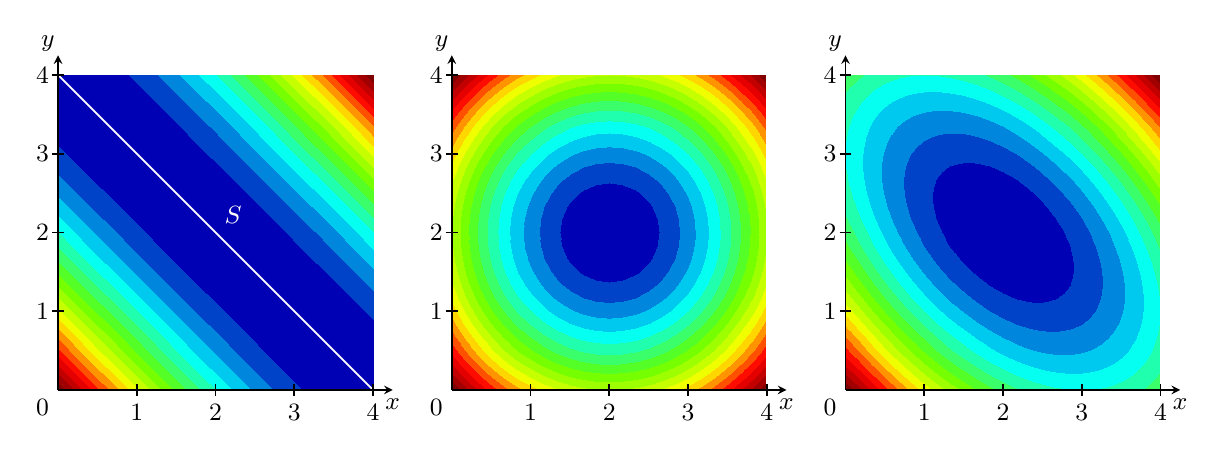
\begin{tikzpicture}[>=stealth, semithick]
            \small\begin{axis}[
                    at = {(0, 0)},
                    domain   = -4:4,   % Domain
                    y domain = -4:4,
                    view     = {0}{90},  % Make it 2D
                    colormap name   = bluered, % Colormap
                    %point meta max  = 150, % Max and Min values
                    %point meta min  = 0,
                    ticks   = none,
                    %unbounded coords = jump,
                    %samples = 50,
                    width   = 4cm,
                    height  = 4cm,
                    xmin=-4, xmax=4,
                    ymin=-4, ymax=4,
                    scale only axis,
                    axis line style={draw=none},
                ]
                \addplot3[
                    contour filled={number=20, labels=false}, semithick
                ]{
                    1/2*(x+y)^2
                };
            \end{axis}
            \begin{axis}[
                    at = {(5cm, 0)},
                    domain   = -4:4,   % Domain
                    y domain = -4:4,
                    view     = {0}{90},  % Make it 2D
                    colormap name   = bluered, % Colormap
                    %point meta max  = 150, % Max and Min values
                    %point meta min  = 0,
                    ticks   = none,
                    %unbounded coords = jump,
                    %samples = 50,
                    width   = 4cm,
                    height  = 4cm,
                    xmin=-4, xmax=4,
                    ymin=-4, ymax=4,
                    scale only axis,
                    axis line style={draw=none},
                ]
                \addplot3[
                    contour filled={number=20, labels=false}, semithick
                ]{
                    x^2+y^2
                };
            \end{axis}
            \begin{axis}[
                    at = {(10cm, 0)},
                    domain   = -4:4,   % Domain
                    y domain = -4:4,
                    view     = {0}{90},  % Make it 2D
                    colormap name   = bluered, % Colormap
                    %point meta max  = 150, % Max and Min values
                    %point meta min  = 0,
                    ticks   = none,
                    %unbounded coords = jump,
                    %samples = 50,
                    width   = 4cm,
                    height  = 4cm,
                    xmin=-4, xmax=4,
                    ymin=-4, ymax=4,
                    scale only axis,
                    axis line style={draw=none},
                ]
                \addplot3[
                    contour filled={number=20, labels=false}, semithick
                ]{
                    1/sqrt(2)*((x+y)+x)*x+1/sqrt(2)*((x+y)+y)*y
                };
            \end{axis}
            \draw[white] (4, 0) -- (0, 4) node[above right, pos=0.5] {\(S\)};
            \node[below left] at (0, 0) {0};
            \node[below left] at (5, 0) {0};
            \node[below left] at (10, 0) {0};
            \draw (1, 0.075) -- (1, -0.075) node[below] {1};
            \draw (2, 0.075) -- (2, -0.075) node[below] {2};
            \draw (3, 0.075) -- (3, -0.075) node[below] {3};
            \draw (4, 0.075) -- (4, -0.075) node[below] {4};
            \draw (5+1, 0.075) -- (5+1, -0.075) node[below] {1};
            \draw (5+2, 0.075) -- (5+2, -0.075) node[below] {2};
            \draw (5+3, 0.075) -- (5+3, -0.075) node[below] {3};
            \draw (5+4, 0.075) -- (5+4, -0.075) node[below] {4};
            \draw (10+1, 0.075) -- (10+1, -0.075) node[below] {1};
            \draw (10+2, 0.075) -- (10+2, -0.075) node[below] {2};
            \draw (10+3, 0.075) -- (10+3, -0.075) node[below] {3};
            \draw (10+4, 0.075) -- (10+4, -0.075) node[below] {4};
            \draw (-0.075, 1) -- (0.075, 1) node[left=0.75mm] {1};
            \draw (-0.075, 2) -- (0.075, 2) node[left=0.75mm] {2};
            \draw (-0.075, 3) -- (0.075, 3) node[left=0.75mm] {3};
            \draw (-0.075, 4) -- (0.075, 4) node[left=0.75mm] {4};
            \draw (5-0.075, 1) -- (5+0.075, 1) node[left=0.75mm] {1};
            \draw (5-0.075, 2) -- (5+0.075, 2) node[left=0.75mm] {2};
            \draw (5-0.075, 3) -- (5+0.075, 3) node[left=0.75mm] {3};
            \draw (5-0.075, 4) -- (5+0.075, 4) node[left=0.75mm] {4};
            \draw (10-0.075, 1) -- (10+0.075, 1) node[left=0.75mm] {1};
            \draw (10-0.075, 2) -- (10+0.075, 2) node[left=0.75mm] {2};
            \draw (10-0.075, 3) -- (10+0.075, 3) node[left=0.75mm] {3};
            \draw (10-0.075, 4) -- (10+0.075, 4) node[left=0.75mm] {4};
            \draw[->] (0, 0) -- (4+0.25, 0) node[below] {\(x\)};
            \draw[->] (0, 0) -- (0, 4+0.25) node[above left=-1mm] {\(y\)};
            \draw[->] (5+0, 0) -- (5+4+0.25, 0) node[below] {\(x\)};
            \draw[->] (5+0, 0) -- (5+0, 4+0.25) node[above left=-1mm] {\(y\)};
            \draw[->] (10+0, 0) -- (10+4+0.25, 0) node[below] {\(x\)};
            \draw[->] (10+0, 0) -- (10+0, 4+0.25) node[above left=-1mm] {\(y\)};
        \end{tikzpicture}
        \caption{Contour plots of the maps \([-4, 4]^2 \to \mathbb{R}\) defined by \(x \mapsto x^\perp H_0x\), \(x \mapsto x^\perp H_1x\) and \(x \mapsto x^\perp (H_0+H_1)x\), where \(n = 1\), \(H_0 = \ketbra{\phi}{\phi}\) for \(\ket{\phi} = H\ket{0}\) and \(H_1 = E_2\). The contour plot shows the actions of the matrices on their respective eigenspaces. Especially, the changes on the nullspace \(S\) show the way \(H_1\) perturbs the spectrum, following the Nullspace Projection Lemma: \(\gamma(H_0)\) is achieved in \(S\), but by adding \(H_1\) with a nonzero action on \(S\), the lowest eigenvalue is decreased. Yet, \(\gamma(H_1|_S^S) \geq c > 0\) does not give the decrease directly, but it is by a value lower than \(c\), as \(d/(c+d+\norm{H_1}) \in (0, 1)\) and as signified by the \enquote{stretching effect}, observable in the third contour plot, of the associated action of \(H_0+H_1\) on \(S\): \(\gamma(H_0+H_1) < \gamma(H_1|_S^S)\).}
        \label{fig:nullspace_projection_lemma_example_contour_plots}
    \end{figure}

    The Nullspace Projection Lemma thus gives a direct lower bound on the smallest eigenvalue of a Hermitian sum. The criteria are rather straightforward, so we may directly use it for the general research problem presented initially. \Cref{fig:nullspace_projection_lemma_example_contour_plots} illustrates the Lemma for a concrete example, showing that we may directly observe the statement.

    \begin{proof}[Proof {\cite[p. 74]{Childs_2014}}.]
        We directly obtain \(H_0, H_1 \neq 0\) and \(\gamma(H_0+H_1) > 0\), as \(\gamma(\evalat{H_1}{S}) > 0\) and \(\gamma(\evalat{H_0}{S}) = 0\). Let \(\ket{\psi} \in \text{eig}_{\gamma(H_0+H_1)}(H_0+H_1)\) be a ground state of the Hamiltonian sum. Using the associated Rayleigh quotient and the corresponding energy characterizations \cite[pp. 234-235]{Horn}, this may also be expressed as
        \begin{align}
            \bra{\psi}(H_0+H_1)\ket{\psi} = \gamma(H_0+H_1)
        \end{align}
        and also
        \begin{align}
            \bra{\psi}(H_0+H_1)\ket{\psi} = \bra{\psi}H_0\ket{\psi}+\bra{\psi}H_1\ket{\psi}
        \end{align}
        Let \(\Pi_S\) be the eigenprojector onto \(S\).

        \phantom{}

        \emph{Case 1.} \(\Pi_S\ket{\psi} = 0\). Then there is no information to be gained from a part of \(\ket{\psi}\) in \(S\). As \(H_1\) is positive-semidefinite, we obtain by definition \(\bra{\psi}H_1\ket{\psi} \geq 0\), so the target inequality
        \begin{align}
            \gamma(H_0+H_1) = \bra{\psi}(H_0+H_1)\ket{\psi} \geq \bra{\psi}H_0\ket{\psi} \geq \gamma(H_0) \geq d > \frac{cd}{c+d+\norm{H_1}}
        \end{align}
        is obtained, as \(c/(c+d+\norm{H_1}) \in (0, 1)\).

        \phantom{}

        \emph{Case 2.} \(\Pi_S\ket{\psi} \neq 0\). Then \(\ket{\psi} \in \text{span}\{\ket{a}, \ket*{a^\perp}\} \eqqcolon S'\), omitting the outer parantheses, for some fixed \(\ket{a} \in S\) and \(\ket*{a^\perp} \in S^\perp\) due to orthonormal decomposition. The proof can thus first be reduced to determining to a bound of \(\gamma(H_0+H_1)\) in this induced subspace, we then argue about the validity over all of \(\mathbb{C}^N\).

        We determine the action of \(H_0+H_1\) on the two-dimensional subspace \(S'\). Observe \(E_N|_{S'}^{S'} = \ketbra{a}{a}+\ketbra*{a^\perp}{a^\perp}\) and \((H_0+H_1)\ket{a} = H_1\ket{a}\). This gives rise to the computations:
        \begin{align}
            (\ketbra{a}{a}+\ketbra*{a^\perp}{a^\perp})H_1\ket{a} &= \underbrace{\bra{a}H_1\ket{a}}_{\eqqcolon v} \ket{a} + \underbrace{\bra*{a^\perp}H_1\ket{a}}_{\eqqcolon w} \ket*{a^\perp}\\
            (\ketbra{a}{a}+\ketbra*{a^\perp}{a^\perp})(H_0+H_1)\ket*{a^\perp} &= \underbrace{\bra{a}H_0\ket*{a^\perp}}_{=(H_0\ket{a})^\perp\ket*{a^\perp} = 0}\ket{a}+\underbrace{\bra*{a^\perp}H_0\ket*{a^\perp}}_{\eqqcolon x}\ket*{a^\perp}\\
            &+\underbrace{\bra*{a}H_1\ket*{a^\perp}}_{=w^*}\ket{a}+\underbrace{\bra*{a^\perp}H_1\ket*{a^\perp}}_{\eqqcolon y}\ket*{a^\perp}
        \end{align}
        In the following, identify \(H_0+H_1\) with \((H_0+H_1)|_{S'}^{S'}\). This gives
        \begin{align}
            H_0+H_1 = \begin{pmatrix}
                v & w^*\\
                w & x+y
            \end{pmatrix}.
        \end{align}
        As \(H_0\) and \(H_1\) are Hermitian, we have \(v, x, y \geq 0\). Thus, \(H_0+H_1 \in H(2)\) also in the restriction to \(S'\). We compute the necessary eigenvalues using the Sarrus rule, giving the equation
        \begin{align}
            \det((H_0+H_1)-\lambda E_2) &= (v-\lambda)(x+y-\lambda)-|w|^2\\
            &= \lambda^2-(v+x+y)\lambda+v(x+y)-|w|^2 = 0
        \end{align}
        and the solutions
        \begin{align}
            \lambda_\pm = \frac{v+x+y}{2} \pm \sqrt{\frac{v+x+y}{4}-v(x+y)+|w|^2}. \label{restricted_hamiltonian_sum_eigenvalues}
        \end{align}
        We now have, that \(\gamma(H_0+H_1) = \lambda_-\), so we consider the final bounds:
        \begin{align}
            \gamma(H_0+H_1) &= \frac{v+x+y}{2} \left(1-\sqrt{1-\frac{4(v(x+y)-|w|^2)}{(v+x+y)^2}}\right)\\
            &\overset{\ref{final_inequalities_2}}{\geq} \frac{v+x+y}{2} \left(1-\sqrt{1-\frac{4vx}{(v+x+y)^2}}\right)\\
            &\overset{\ref{final_inequalities_3}}{\geq} \frac{vx}{v+x+y} = \frac{1}{\frac{1}{v}+\frac{1}{x}+\frac{y}{vx}}\\
            &\overset{\ref{final_inequalities_4}}{\geq} \frac{cd}{c+d+\norm{H_1}}
        \end{align}
        \begin{enumerate}[label=(\arabic*), wide]
            \item \label{final_inequalities_2} Consider the action of \(H_1\) on \(S'\) in the same way as we did for \(H_0+H_1\). This yields
            \begin{align}
                H_1 = \begin{pmatrix}
                    v & w^*\\
                    w & y
                \end{pmatrix}
            \end{align}
            As \(H_1\) is also positive-semidefinite in its restriction, we by \Cref{lem:positive_semidefiniteness_determinant} obtain, that \(vy-|w|^2 \geq 0\). The associated term in the square root is strictly monotonically descending, giving the inequality.
            \item \label{final_inequalities_3} Since \(\sqrt{1-x} \leq 1-\frac{x}{2}\) for \(x \in [-1, 1]\) \cite[pp. 285-286]{Forster}.
            \item \label{final_inequalities_4} We have three inequalities. First, \(\ket{a} \in S\), so \(v = \bra{a}H_1\ket{a} \geq \gamma(H_1|_S)\), as \(\ket{a} \in S\). Second, \(x = \bra*{a^\perp}H_0\ket*{a^\perp} \geq \gamma(H_0)\). Third, \(y \leq \norm{H_1}\). All three are based on \cite[pp. 234-235]{Horn}. The term is strictly monotonically ascending in \(v\) and \(x\), and strictly monotonically descending in \(y\), allowing the resulting bound.
        \end{enumerate}

        \phantom{}

        The preceding argument can now be applied with arbitrary choices of \(\ket*{a^\perp}\), covering \(\mathbb{C}^N\) in the form
        \begin{align}
            \mathbb{C}^N = \bigcup_{\substack{\ket*{a^\perp} \in S(\mathbb{C}^N)\\\ket*{a^\perp} \perp \ket{a}}} \text{span}\{\ket{a}, \ket*{a^\perp}\},
        \end{align}
        giving the statement.
    \end{proof}

    We make the following remarks.
    \begin{itemize}[wide]
        \item I may note that I initially had trouble with the validity of the proof because of the reduction to the two-dimensional subspace with a fixed orthonormal decomposition. The argument at the end gives the validity and works in many such applications of this proof technique, take for instance the standard runtime proof for the adiabatic Grover algorithm \cite[pp. 8-10]{Albash_2018}.
        \item There is a mistake in the proof as presented in the original paper. \(\ket{\phi} \in \ker(H_0+H_1)\) does not imply \(\ket{\phi} \in S\). See e.g. \(H_0 = -\ketbra{0}{0}\) and \(H_1 = E_2\). Then \(\ket{0} \in \ker(H_0+H_1)\), as \(H_0+H_1 = \ketbra{1}{1}\), but \(\ket{0} \notin S\). Additionally, this leads onto a small paragraph ending with a Rayleigh quotient formula in the second line before equation (E.3), which is never used. These claimed facts are never used either.
        \item The well-definedness of the solutions in \Cref{restricted_hamiltonian_sum_eigenvalues} implies multiple inequalities.
    \end{itemize}

    Furthermore, we observe, that switching the order of \(H_0\) and \(H_1\) in the original statement makes the use for AQC algorithms easier, as \(H_0\) is usually seen as the target Hamiltonian to evolve to in the AQC algorithm. \(H_1\) should be the initial Hamiltonian, as its adjustment may lead to a better bound of the lowest eigenvalue of the Hermitian sum. We thus state the same Lemma again with switched symbols.

    \begin{theorem}[{Nullspace Projection Lemma (Alternative Formulation) \cite[p. 73]{Childs_2014}}]
        Let \(H_0, H_1 \in H(N)\) be positive-semidefinite. Suppose \(S \coloneqq \ker(H_1) \neq \emptyset\) and let \(c, d \in \mathbb{R}_{> 0}\), s.t.
        \begin{align}
            \gamma(H_1|_S^S) \geq c > 0 \text{ and } \gamma(H_1) \geq d > 0.
        \end{align}
        Then
        \begin{align}
            \gamma(H_0+H_1) \geq \frac{cd}{c+d+\norm{H_0}}.
        \end{align}
    \end{theorem}

    \paragraph*{\textbf{Application}} In the following, we apply the Nullspace Projection Lemma to the adiabatic Grover algorithm \cite[pp. 8-10]{Albash_2018} to demonstrate its practicability on one example. We use the following adjusted setting: We seek an element \(m \in [0, N-1]_{\mathbb{N}}\) encoded in the final Hamiltonian of the path
    \begin{align}
        H(s) \coloneqq (1-s)(E_N-\ketbra{\phi}{\phi})+s(2E_N-\ketbra{m}{m}) \eqqcolon (1-s) H_0 + s H_1
    \end{align}
    with \(\ket{\phi} \coloneqq H^{\otimes n}\ket{0}^{\otimes n}\). We wish to use the alternative formulation of the Nullspace Projection Lemma. We have the spectra \(\sigma(H_0) = \{0, 1\}\) and \(\sigma(H_1) = \{1, 2\}\), as well as the nullspace \(S = \text{span}\{\ket{m}\}\). \(H_0\ket{m} = \ket{m} - \frac{1}{\sqrt{N}} \ket{\phi}\), so we have \(\sigma(H_0|_S^S) = \{1-\frac{1}{N}\}\). Plugging \(c \coloneqq 1-\frac{1}{N}\) and \(d \coloneqq 1\), as well as \(\norm{H_0} = 1\) into the Nullspace Projection Lemma, we obtain for any time point \(s \in (0, 1)\)
    \begin{align}
        \gamma(H(s)) \geq \frac{(1-s)\left(1-\frac{1}{N}\right)s}{(1-s)\left(1-\frac{1}{N}\right)+s+1} = \frac{s}{1+\frac{(s+1)N}{(1-s)(N-1)}} > s,
    \end{align}
    as \(\sigma(\alpha H') = \alpha \sigma(H')\) for any Hamiltonian \(H' \in H(N)\) and \(\alpha \in \mathbb{R}\).

    \printbibliography{}
\end{document}
